Основной особенностью отображения трехмерной графики в веб среде является невозможность прямого доступа к аппаратному обеспечению
посредством низкоуровневых графических библиотек, таких как OpenGL или Vulkan (Direct 3D в данной работе не рассматривается ввиду
проприетарности технологии) так как основная среда выполнения пользовательского кода в браузерах - виртуальная машина javascript,
не позволяющая пользовательскому коду использовать критические ресурсы компьютера.

Одной из технологий, позволяющей отображение трехмерной графики в браузере, является WebGL -- клиентская технология, построенная на базе
WebAssembly, платформы для разработки клиентских приложений с помощью native языков. WebAssembly -- также известный под названиями WA
или Wasm -- является платформой для выполнения низкоуровневого байт-кода, предназначенной для исполнения в браузере. В данный момент находится
на стадии разработки. Первоначальной целью была поддержка С/С++, хотя уже сейчас поддерживается Rust, и также в дальнейшем предполагается
поддержка других языков. WebAssemblу представляет собой переносимое абстрактное синтаксическое дерево, обеспечивающее как более быстрый парсинг,
так и более быстрое выполнение кода, чем JavaScript\cite{js_web}. Изначально WebAssembly основывался на asm.js и PNaCl. Команда, работающая над WebAssembly,
включает разработчиков из компаний Mozilla, Google, Microsoft и Apple, которые представляют на рынке четыре наиболее распространённых браузера — Firefox,
Chrome, Microsoft Edge и Safari соответственно.

WebGL — это контекст элемента canvas HTML, который обеспечивает API 3D графики без использования плагинов. Вся работа веб-приложений с использованием WebGL основана на коде JavaScript.
За счёт использования низкоуровневых средств поддержки OpenGL, часть кода на WebGL может выполняться непосредственно на видеокартах., благодаря чему разработчики могут получить доступ
к дополнительным ресурсам компьютера, увеличивая быстродействие работы приложений.
Таким образом, для создания приложений можно использовать стандартные для веб-среды технологии HTML/CSS/JavaScript и при этом также применять аппаратное ускорение графики.
Часто создание настольных приложений работающих с 2d и 3d-графикой нередко ограничивается возможностями целевой платформой, то здесь главным ограничением является только поддержка
браузером технологии WebGL. 
WebGL возник из экспериментов над Canvas 3D американского разработчика из компании Mozilla в 2006 году. Впоследствии разработчики браузеров Opera и Mozilla стали создавать свои
реализации WebGL. А впоследствии была организована рабочая группа с участием крупнейших разработчиков браузеров Apple, Google, Mozilla, Opera для работы над спецификацией
технологии. И в 3 марта 2011 года была представлена спецификация WebGL 1.0.

Использование WebAssembly позволяет пользовательскому коду, написанному на JavaScript потреблять API, реализованный низкоуровневыми библиотеками, реализованными
на языках C/C++ со скоростью, сравнимой со скоростью их выполнения в обычном приложении для рабочего стола. В дальшейнем, отрендеренную аппаратными средствами
текстуру можно отобразить на html5 canvas и интегрировать в веб-документ.

Для отображения трехмерной графики можно использовать один из нижеуказанных стеков технологий.
Для реализации логики приложения на основе стека Mono/.NET или cPython, можно использовать следующий подход:
\begin{enumerate}[label=\arabic*.]
\item Высокоуровневый движок рендеринга трехмерной графики, например Godot или Unity3D с поддержкой сборки для WebGL (\ref{figure:domain:webgl})
\item Unity/Godot WebPlayer для интерпретации логики приложения 
\item Библиотека трехмерной графики Three.js.
\item Реализация OpenGL для Web - WebGL.
\item WebAssembly и Emscripten для обращения к низкоуровневым графическим API OpenGL.
\item Реализация графического API OpenGL для C.
\end{enumerate}

\begin{figure}[ht]
\centering
  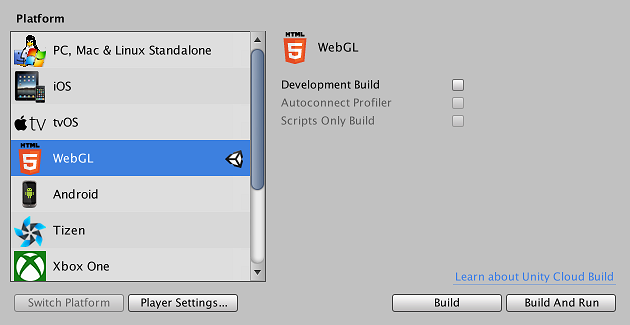
\includegraphics[scale=1.25]{webgl_build_unity.png}
  \caption{Инструменты для сборки Unity WebGL проекта}
  \label{figure:domain:webgl}
\end{figure}

Данный подход позволит реализовать одностраничное веб приложение, отображающее Godot или Unity3D проект в браузере, и по своей природе напоминает Flash-based SPA.
Для реализации веб приложения в виде классического веб сайта возможно использование того же стека технологий начиная с Three.js. В таком случае над графическим
приложением необходима реализация веб-приложения-обертки, которое разрабатывается на привычном для Web стеке технологий -- JavaScript, TypeScript, Dart:
\begin{enumerate}[label=\arabic*.]
\item Библиотека трехмерной графики Three.js а также управляющий приложением JavaScript или TypeScript код.
\item Реализация OpenGL для Web - WebGL.
\item WebAssembly и Emscripten для обращения к низкоуровневым графическим API OpenGL.
\item Реализация графического API OpenGL для C.
\end{enumerate}

